% (c) 2020 Stefan Antonowicz
% Based off of tex found at https://github.com/ludus-leonis/nipajin
% This file is released under Creative Commons Attribution-NonCommercial-ShareAlike 4.0 International License.
% Please do not apply other licenses one-way.

\renewcommand{\yggCivilization}{%
  \mychapter{Civilization}{civilization}
}

\renewcommand{\yggCivilizationText}{%


  \mysection{Weights and Measures}{civilization-weights-and-measures}


  \mysubsection{Money}{civilization-money}
  The Totality of Ygg subscribes to a Chartalist approach to economy.  Acheron in particular is an amalgam of multiple civilizations built on the bones of the civilizations before them, stretching back 30,000 years or more.  The rarity of certain metals (silver and gold), as well as the utility of another (iron) has created an easy way to measure credit and debt.  A 5,000 year old gold coin found in a crypt and another minted by the city of Byzantium have the same value; iron, silver, and gold are the uniform system for measuring credits and debts and have remained so for millenia.  

  Thus, coins are divided into 3 types - iron (fe), silver (ag), and gold (au) - and have the following value relative to one another

  \example{
    100 fe (iron) = 10 ag (silver) = 1 au (gold)
  }



  Iron is the core of the monetary system, specifically the iron ingot (1kg of iron), which is equal to 100 iron coins.  It is not uncommon for iron coins to be smelted to forge the tools, weapons, and armor they pay for (particularly when various cities are trying to feed and arm their military).  

  \cbreak

  Ingots of each type are common, and weigh 1kg each.  Every ingot you find is worth 100 of the coin type:
  \mybullet {
    \item 1 iron ingot = 1kg iron = 100fe (iron pieces)
    \item 1 silver ingot = 1 kg silver = 100ag (silver pieces)
    \item 1 gold ingot = 1 kg gold = 100au (gold pieces)
  }

  4 1kg ingots / 400 coins count as 1 \mylink{Burden}{gear-burden}.

  \myhighlight{Coins}{civilization-coins}

  Whenever you see "coins" instead of a coin type, this means a coin appropriate to your \LVL.  Levels 1-2 are the Iron levels (fe), levels 3-5 are the Silver levels (ag), and levels 6+ are the Gold levels (au)

  \begin{center}
  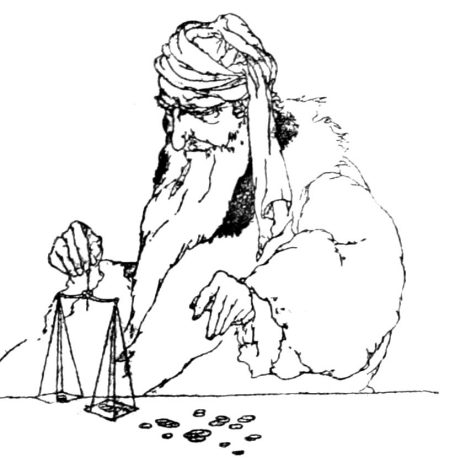
\includegraphics{Moneychanger}
  \end{center}


\newpage

  \mysection{Settlements}{settlements}

  Acheron is dominated by wide, unpopulated wastes filled with ruins, dangers, and uncovered riches; the people of Acheron cluster in various settlements that dot the landscape.  These settlements are broken into 4 sizes

  \mylist {
    \item \mybold{Tiny}  Thorps, dorfs, "the boondocks" (< 1,000 people).  A Tiny Settlement may have a few things people might trade for, and you'll probably sleep in a hayloft for a day or two at the most before someone chases you off.  Tiny settlements only deal in trade, and \myital{maybe} a few iron pieces.  They are generally superstitious and uneducated (see \mylink{Burn the Witch!}{mystic-complication-witch}).  \mybold{You cannot take a Vacation in a Tiny settlement}


    \item \mybold{Small (Iron)}
    Hamlets (1,000 - 10,000 people).   The "iron" settlements. Small settlements generally deal in iron - if you attempt to spend silver in a Small settlement, you might meet with some strange looks and attract unwanted attention.  Trying to spend gold in a Small settlement is pretty much impossible.

    \item \mybold{Medium (Silver)}
    Villages, wyches and small towns (~10,000 to ~100,000 people).  The "silver" settlements. Medium settlements usually deal in silver, though gold is sometimes used by the wealthy and iron used by the impoverished.  

    \item \mybold{Large (Gold)}
    Big towns and cities (100,000+ people).  The "gold" settlements.  Large settlements deal almost entirely in gold.  Trying to spend iron pieces in a metropolis would be met with disdain, like trying to pay your cab fare with pennies (and unlike modern civilization, no one is under any obligation to honor your tender if they don't feel like it).
  }

  The size of the settlement is important when it comes to longer rests, spending treasure, and finding \mylink{equipment}{equipment}, \mylink{services}{civilization-services}, and \mylink{hirelings}{gear-hirelings}.

  \cbreak

  \mysubsection{Taking a Vacation}{civilization-vacation}
  
  In order to truly recuperate, you must return to Civilization and rest in a Small, Medium, or Large settlement. You tell the Arbiter how long of a Vacation you're taking: Days, Weeks, or Months. Taking a Vacation costs money.  The costs shown are for food, lodging, equipment maintenance, Trope and Species specific stuff (whetstones, lockpicks, trap kits, inks, paper, weird bones, blood tokens, esoteric pieces of art, edible moss, rats-on-sticks, guild dues, etc.) and simple diversions of all types.  These are only the basics, however - with all that coin in your pocket you may want to go \mylink{Carousing}{advancement-carousing}. 

  If you don't have the money, you don't get any of the benefits of the longer rest.

  \mytable{X c c c}{
    \thead{} & \thead{Small} & \thead{Medium} & \thead{Large} \\
  }{
    Vacation & 100 \FE & 50 \AG & 25 \AU \\
  }

  During a Vacation, you:

  \mybullet {
    \item Restore all your Grit and Flesh
    \item Go Carousing (appropriate to your level)
    \item Restore your Armor \UD up to its \MAX. See the section on \mylink{Armor Repair}{gear-armor-repair} for how to restore the \MAX
    \item Restore your \UD for all Intangible Stats up to their \MAX
    \item Restore all Deed \UD (Sellswords)
    \item Restore all Luck \UD (Knave and Pooka)
    \item Restore all Blood \POOL (Sorcerers)
    \item Restore all Mojo \UD
    \item Restore all Grace \POOL (Mystics)
    \item Restore all Remembrance (Spriggan)
  }

  \cbreak

  In addion, you can do the following (explained in detail in \mybold{Bell, Book, \& Candle}:

  \mybullet {
    \item  Perform Research and Marvels, or create Wonders
    \item  Cure Disease, remove Addiction, or expel a curse
    \item  Heal a Beating, Madness, or Life Drain
  }

  \cbreak

  \begin{center}
  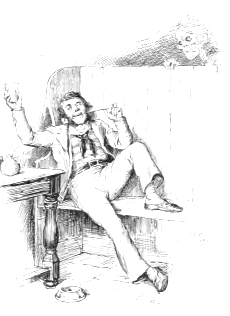
\includegraphics{Vacation}
  \end{center}



  \newpage
  \end{multicols}

  \mysubsection{Services}{civilization-services}
  
  Not all Settlements have all the services an adventurer may require:

  \mybullet {
    \item You'll need a Trader to buy \mylink{Adventuring Gear}{gear-adventuring}; otherwise, there's only a 1-in-6 chance that the Settlement has something you're looking for (including weapons and armor if a Leatherworker or Smith isn't present)
    \item You'll need a Leatherworker to \mylink{buy or repair Light Armor}{gear-armor-repair}
    \item You'll have to pay a Smith to \mylink{buy or repair Medium or Heavy Armor}{gear-armor-repair}, or to buy \mylink{weapons}{gear-weapons}
    \item Not all Settlements have shrines or chapels to specific Small Gods, so their worshippers may not be present
    \item You'll need to know if there's an apothecary or ... less savory type ... who can sell you \mylink{Narcotics}{gear-narcotics} 
    \item You'll need a Library in order to use Research (Chymistry, Inscription, and Medicinals)
    \item You'll need a Sanitarium in order to use Research on Medicinals (if a Library isn't present)
    \item If you don't have access to Medicinals or a Hekaphage, you'll need a Miracle Worker (wisewoman, witch, chymist, apothecary, leech, etc) to cure Disease; remove Addiction; expel a Curse; or heal a Beating, Madness, or Life Drain
  }


  These are the basic odds of you finding a service you need are an x-in-6 (for example, if you see 2-in-6, that means the service is present if you  roll a 1 or a 2 on a d6).

  The Arbiter can feel free to ignore these results if she chooses!

  \mytable{X c c c c}{
    \thead{} & \thead{Tiny} & \thead{Small} & \thead{Medium} & \thead{Large} \\
  }{
    Trader? & 1-in-6 & 4-in-6 & 6-in-6 & 6-in-6 \\
    Leatherworker? & 1-in-6 & 4-in-6 & 6-in-6 & 6-in-6 \\
    Smith? & No & 1-in-6 & 6-in-6 & 6-in-6 \\
    Shrine to a specific Small God? & No & 1-in-6 & 3-in-6 & 6-in-6 \\
    Library? & No & 2-in-6 & 4-in-6 & 6-in-6 \\
    Narcotics? & No & \MAX-in-6 & 6-in-6 & 6-in-6 \\
    Sanitarium? & No & 1-in-6 & 3-in-6 & 6-in-6 \\
    Miracle Worker? & 6-in-6 & 5-in-6 & 4-in-6 & 3-in-6 \\
  }

    \begin{center}
  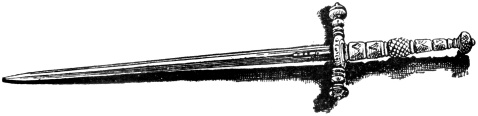
\includegraphics{Dagger}
  \end{center}


  \newpage

  \begin{multicols}{2}



  \mysection{Languages}{civilization-languages}

  A number of dialects and idiolects are used across the surface of the Totality.
  
  \mysubsection{Dialects}{civilization-dialects}

  \myhighlight{Acheron}{dialect-acheron}

  Common language of the Totality of Ygg.  Everyone can speak this.

  \myhighlight{Baroque}{dialect-baroque}

  Native language of the Amaranthine Kingdoms of Byzantium

  \myhighlight{Brogue}{dialect-brogue}

  Language of the people of the Grim Wood in Blackmoor


  \myhighlight{Cockney}{dialect-cockney}

  Slang used by thieves, merchants, slave traders, etc - favored by residents of Ophir, Lankhmar, Ilthmar, Quarmall, etc.

  \myhighlight{Kaddish}{dialect-kaddish}

  Native language of the Immortal Empire of Yoon-Suin

  \myhighlight{Kleshian}{dialect-kleshian}

  Language of the Jungles of Klesh. There's no written component - spoken only

  \myhighlight{Mingol}{dialect-mingol}

  The language of the Steppe of Khitai and the Plain of Sifir

  \myhighlight{Saltish}{dialect-saltish}

  Native language of the Free Confederacy of Sea Princes

  \myhighlight{Sibilance}{dialect-sibilance}

  The language used around Elfland, the Lands of Nod, and the Weald.  All Zoological creatures can speak Sibilance by the grace of the King of Elfland (though you might not get much of an answer out of them)

  \myhighlight{Skaldic}{sdialect-kaldic}

  Language of the people of the Taiga, Nin, and Vornheim


\mysubsection{Idiolects}{idiolects}

\myhighlight{Archaic}{idiolect-archaic}

Required to command extraplanar Archons

\myhighlight{Birdsong}{idiolect-birdsong}

The language of hearth spirits, ravens, and daytime birds.  Said to be a common language in the Ultraviolet Grasslands and the Plateau of Leng

\myhighlight{Bloodspeech}{idiolect-bloodspeech}

A series of cries and hand signals for communicating in the battlefield

\myhighlight{Draconic}{idiolect-draconic}

Language of the Night Children and intelligent reptiles (like dragons).  Said to be spoken by the folk who dwell in the Eiglophian Mountains as well.

\myhighlight{Fiendish}{idiolect-fiendish}

Required to command extraplanar Fiends

\myhighlight{Graveborn}{idiolect-graveborn}

Language of intelligent undead.   Required to speak with the dead.  Said to be a language understood by the ghosts that inhabit the Lost Cities

\myhighlight{Seraphic}{idiolect-seraphic}

Required to command extraplanar Seraphim

\myhighlight{Sylvan}{idiolect-sylvan}

Language of intelligent/magical animals and members of the court of the King of Elfland

\myhighlight{Thieves Cant}{idiolect-thieves-cant}

Language spoken by thieves found across the continent

\myhighlight{Silent Speech}{idiolect-silent-speech}

Language of the Veins of the Earth, stones, and rocks

\myhighlight{Verminish}{idiolect-verminish}

Language or insects, rats, and other vermin. A gift from the Rat God to Acheron


} %end
